\documentclass[letterpaper, 10 pt, conference]{ieeeconf}
\overrideIEEEmargins
\IEEEoverridecommandlockouts                   
\usepackage{times}
\usepackage{multicol}
\usepackage{graphicx}
\usepackage{xcolor}

% \usepackage{hyperref}

\usepackage{amsmath}
\usepackage{amssymb}
\newtheorem{theorem}{Theorem}
% \usepackage{lmodern}

\usepackage[algoruled,vlined,linesnumbered]{algorithm2e}
\usepackage{anyfontsize}


\title{CPS$\_$S MATH 453 Final project: Your Title}

\author{firstname1 lastname1, firstname2 lastname2 
}



\begin{document}

\maketitle

\begin{abstract}

----

\end{abstract}




\section{Introduction}

This section sets the stage for your research. It typically includes the background information on the topic, the context of the study, and the significance of the research. The introduction ends with a clear statement of the question or hypothesis that the paper aims to address.
asdfasf
 \begin{figure}
 \centering
 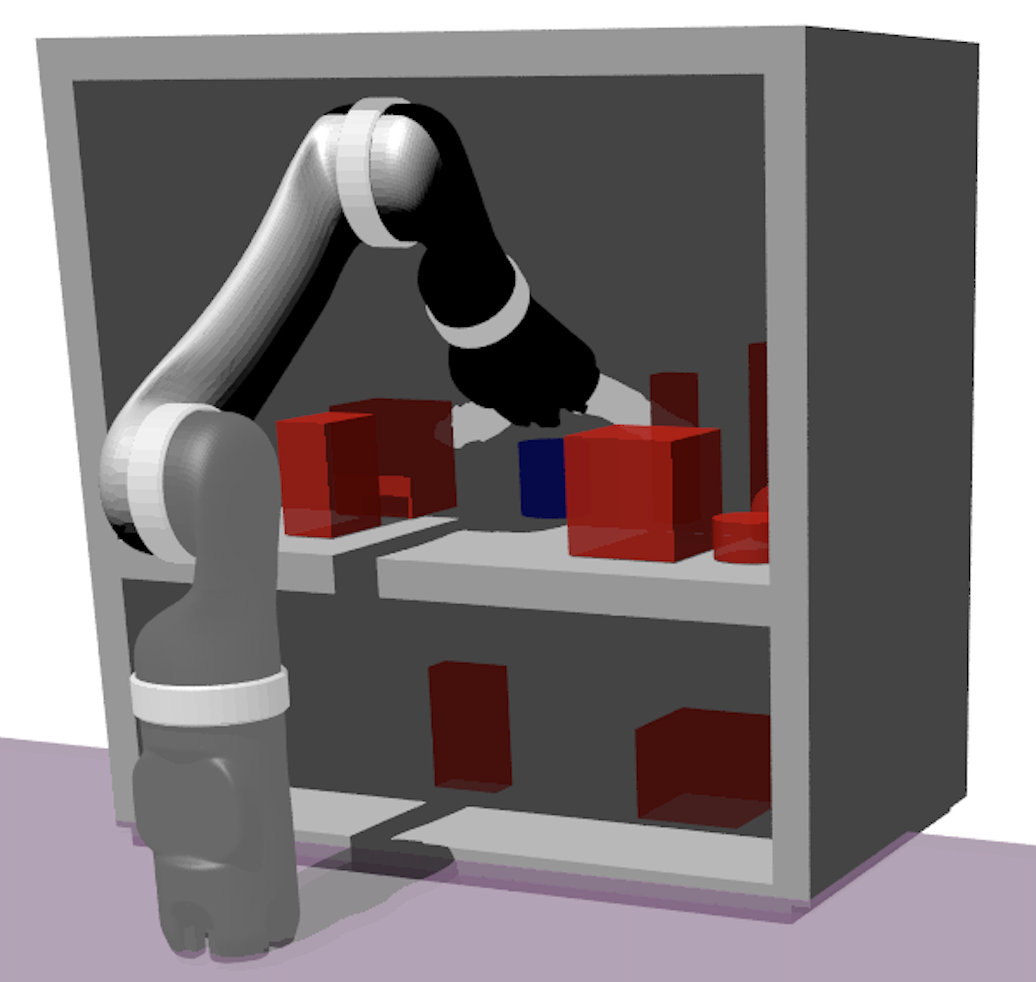
\includegraphics[width=0.4\textwidth]{figures/blocking.png}
      \caption{Figure example}
\label{fig:example}
\end{figure}

\emph{Statement of your question.}
%

\section{Related work}
You can add your references here. For example: \cite{McGeer01041990}

\section{Problem Formulation}
Here, you define and clarify the specific problem or issue your research is tackling, including, the input to the problem, and the expected output of the problem. 
For the project proposal, please ensure that you complete all sections up to and including this one.

\section{Algorithm/Methodology}
This part describes the algorithms and the methods used to solve the proposed problem. It should provide enough detail so that others can clearly understand what you did. 

\section{Experiments/Results}
In the results section, you present the experiments you run and any results/findings of your experiments. This section includes data, often in the form of tables, graphs, or charts, and a narrative that describes the data objectively.

\bibliographystyle{IEEEtran}
\bibliography{IEEEabrv, references}

\end{document}

